\documentclass{beamer}

\usepackage[utf8]{inputenc}
\usepackage[T1]{fontenc}

\usepackage{xcolor}
\definecolor{darkgreen}{rgb}{0,0.6,0}
\usepackage[scaled=0.8]{beramono}

% \usepackage[euler-digits]{eulervm}
%\usefonttheme[onlymath]{serif}

\usepackage{listings}
% \usepackage{amsmath}
% \usepackage{amssymb}
% \usepackage{oz}
% \usepackage{mathpartir}
% \usepackage{cancel}
% \usepackage{graphbox}

% \input{macros}
\usepackage{./why3lang}
\lstset{basicstyle={\ttfamily\footnotesize}}

% \input{options}
\newcommand{\why}{\lstinline[language=why3]}


\setbeamertemplate{navigation symbols}{}%remove navigation symbols
% \setbeamercolor{footline}{fg=blue}
% \setbeamerfont{footline}{family=\sffamily}
% \setbeamertemplate{navigation symbols}{%
%     \usebeamerfont{footline}%
%     \usebeamercolor[fg]{footline}%
%     \hspace{1em}%
%     \insertframenumber/\inserttotalframenumber
% }

\usepackage{tikz}
\usetikzlibrary{shapes,arrows,shadows,backgrounds}
\tikzstyle{bloc} = [rectangle, draw, fill=green!30,
     text centered, rounded corners]
\tikzstyle{tool} = [rectangle, draw, fill=red!30,
    text centered]
\tikzstyle{blocl} = [rectangle, draw, color=black!50, fill=green!10,
     text centered, rounded corners]
\tikzstyle{tooll} = [rectangle, draw, color=black!50, fill=red!10,
     text centered]
\tikzstyle{line} = [draw, -triangle 45]
\tikzstyle{linel} = [draw, color=black!50,-triangle 45]
\tikzstyle{elem} = [ellipse, draw, top color=green!5, bottom color=green!30,
     text centered, rounded corners, drop shadow]
\tikzstyle{newtool} = [tool, dashed, top color=blue!10, bottom color=blue!40]
\tikzstyle{newelem} = [elem, dashed, top color=green!10, bottom color=green!40]
\tikzstyle{lib} = [rectangle, draw, top color=yellow!4, bottom color=yellow!30,
    text centered, rounded corners, drop shadow, shading=axis]

\usetikzlibrary{decorations.text}

\setbeamertemplate{blocks}[rounded][shadow=true]
\setbeamercolor{block title}{bg=green!20}
\setbeamercolor{block body}{bg=green!10}
\setbeamercolor{block title alerted}{bg=red!20}
\setbeamercolor{block body alerted}{bg=red!10}
\setbeamercolor{block title example}{bg=blue!20}
\setbeamercolor{block body example}{bg=blue!10}

%\usepackage{./why3lang}

%\input{../../../talks/latex/macros-slides-claude}
%\lstnewenvironment{whycode}{\lstset{language=why3}}{}
% \lstnewenvironment{whycodesmall}{\lstset{language=why3}\lstset{basicstyle={\ttfamily\footnotesize\color{blue}}}}{}
% \lstnewenvironment{ocamlcode}{\lstset{language={[Objective]Caml}}}{}
% \newcommand{\of}[1]{\lstinline[framesep=0pt]{#1}}
% \lstset{basicstyle={\ttfamily\small}}

% \definecolor{test}{rgb}{.95,.45,.65}
% \definecolor{myblue}{rgb}{0.25,0.41,0.88}

\definecolor{links}{HTML}{2A1B81}
\hypersetup{colorlinks,linkcolor=,urlcolor=links}

\let\oldemph\emph\renewcommand{\emph}[1]{\oldemph{\color{blue} #1}}
\let\oldtexttt\texttt\renewcommand{\texttt}[1]{\oldtexttt{\color{black} #1}}
\newcommand{\m}[1]{\(\color{darkgreen}#1\)}
\newcommand{\mm}[1]{\[\color{darkgreen}#1\]}
\newcommand{\cit}[1]{\hfill{\color{darkgreen}[#1]}}


 \titlegraphic{
%   \includegraphics[width =0.18\textwidth]{../images/logo-why3-hires.png} \hfill
%   \includegraphics[width =0.2\textwidth]{../images/proofinuse.png}
   \fbox{Ceci n'est pas le logo de Décysif}
  }

\newcommand{\expapprox}{\widehat{\exp}}
\renewcommand{\lnapprox}{\widehat{\log}}
\newcommand{\experror}{E_{\exp}}
\newcommand{\lnerror}{E_{\log}}
\newcommand{\expmax}{M_{\exp}}
\newcommand{\lnmax}{M_{\log}}
\newcommand{\lseapprox}{\widehat{\lse}}
\newcommand{\lse}{\textsf{LSE}}
\newcommand{\slse}{\textsf{SLSE}}
\newcommand{\err}{\varepsilon}
\renewcommand{\ln}{\log}

\title{Livrables 1.1 et 2.1 (jeux de tests) \\
  Overview de ``why3 bench'' et ``why3 session''\\
  Quelques propositions}

\author{Claude~Marché\inst{1}}

\institute{\inst{1} Université Paris-Saclay, Inria \& LMF }

\date{Décysif, 6 février 2024}

\begin{document}

\lefthyphenmin=30

\begin{frame}{}
  \maketitle
\end{frame}


\begin{frame}{Objectifs}

  \begin{block}{L1.1. (resp: TrustInSoft)}
    Constitution d’une base de fichiers d’entrée représentatifs des
    difficultés rencontrées pour générer des exploits.
  \end{block}

  \begin{block}{L2.1. (resp: AdaCore)}
    Constitution d’une base de fichiers d’entrée représentatifs des
    difficultés rencontrées pour la preuve automatique.
  \end{block}

\end{frame}

\begin{frame}{Nouveautés récentes (Why3)}

  \begin{block}{Format de fichier ``S-expression''}
    Garantie de conformité de la chaîne
    \begin{center}
    PTree $\mapsto$ printer
    $\mapsto$ fichier .sexp $\mapsto$ re-parsing $\mapsto$ Ptree
  \end{center}
  \end{block}


  \begin{block}{\texttt{why3 bench}}
    \begin{itemize}
    \item Execution d'un ensemble de prouveurs sur un jeu de tests
      (en \why{.mlw} ou en \why{.sexp})
    \item Execution interruptible en cas de gros jeu de données
    \end{itemize}

  \end{block}

  \begin{block}{\texttt{why3 session info -{}-stats -{}-graph}}
    \begin{itemize}
    \item Statistiques sur les résultats, graphiques
    \end{itemize}

  \end{block}

\end{frame}


\begin{frame}[fragile]{Exemple: Z3 option \texttt{-{}-nombqi}}

\begin{lstlisting}
> why3 session info --provers-stats sessions/*/*.xml sessions/*/*/*.xml
381 session(s) read, with a total of 40898 proof goals.
== Statistics per prover: number of proof attempts, successful ones, time (minimum/maximum/average) in seconds ==
  Z3 4.12.2                     : 40898 30776   0.00   4.81   0.07
  Z3 4.12.2 (nombqi)            : 40898 30773   0.00   4.78   0.07
\end{lstlisting}

\end{frame}


\begin{frame}{Exemple: Z3 \texttt{-{}-nombqi} avec \texttt{-{}-graph=hist}}

  \begin{center}
    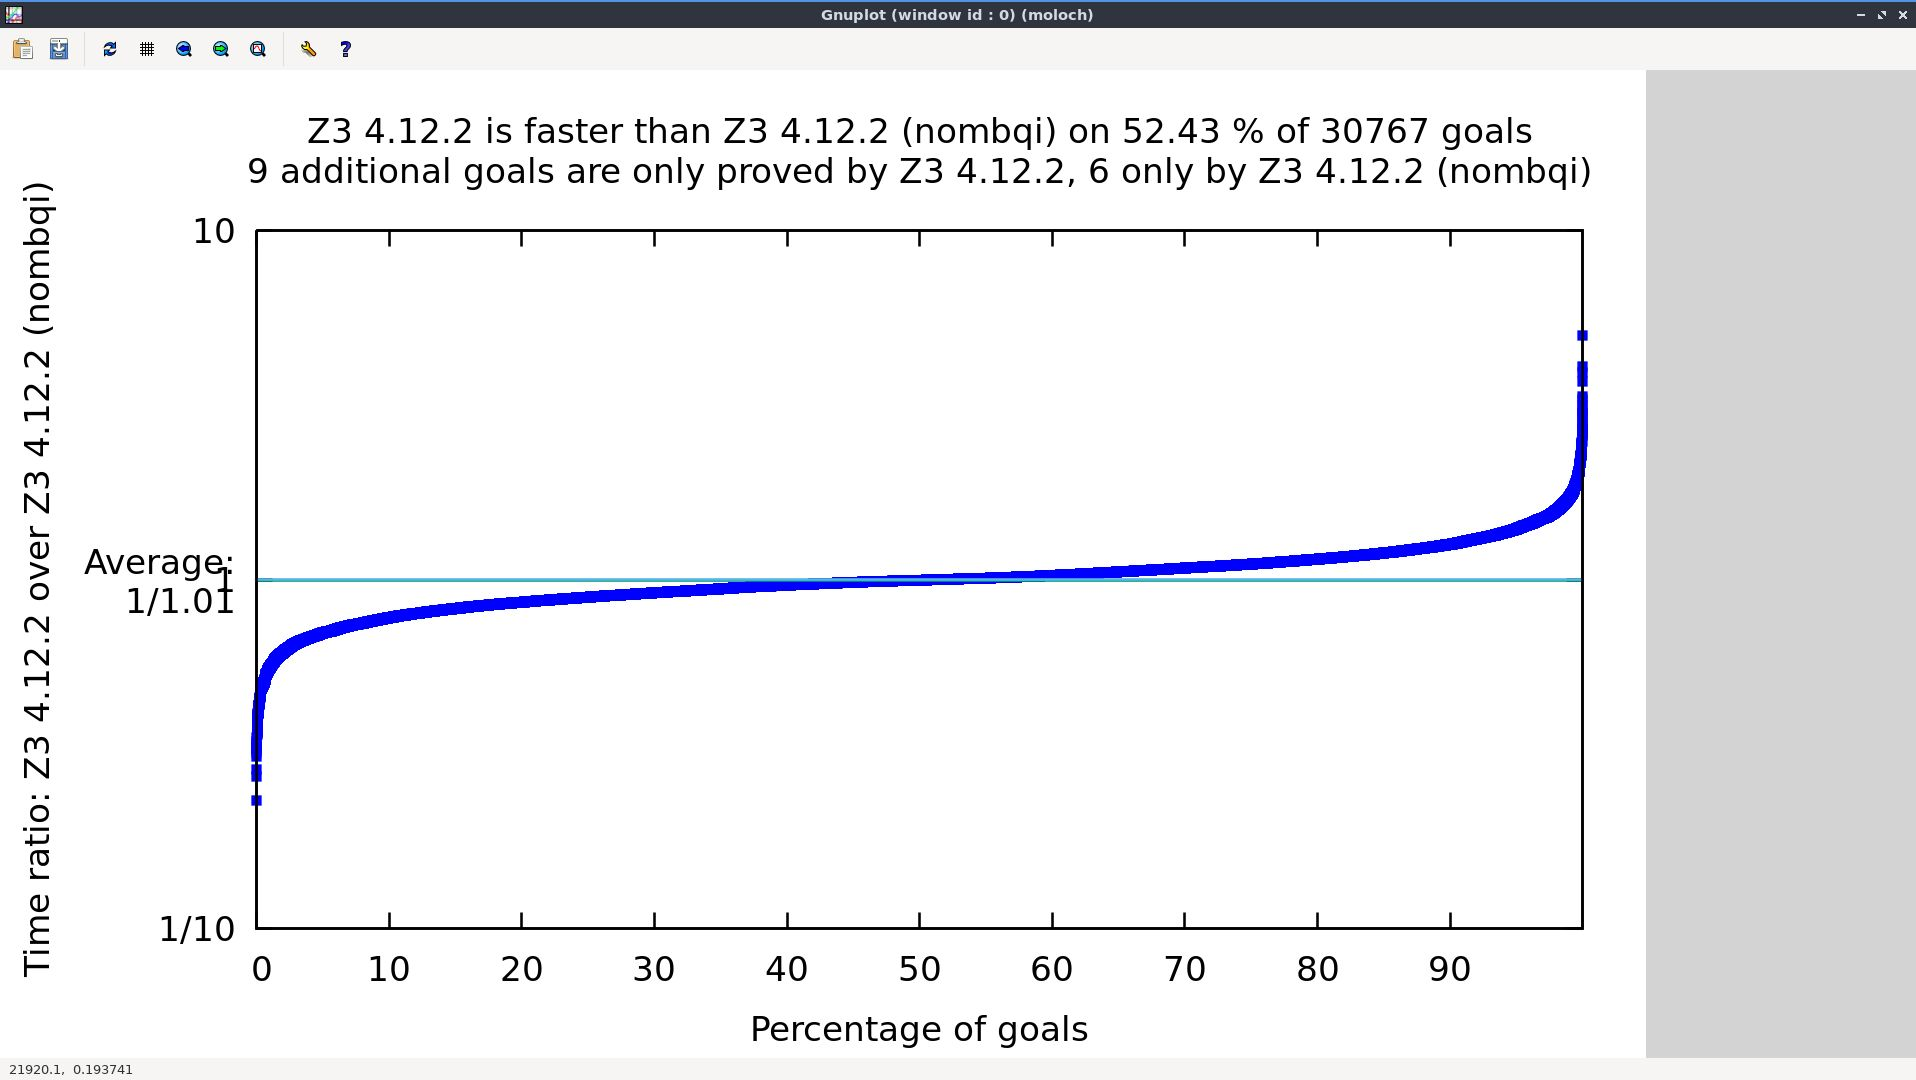
\includegraphics[width=\textwidth]{z3_nombqi.jpg}
  \end{center}

\end{frame}

\begin{frame}{Autre exemple: Alt-Ergo 2.5 ``Dolmen''}

  \begin{center}
    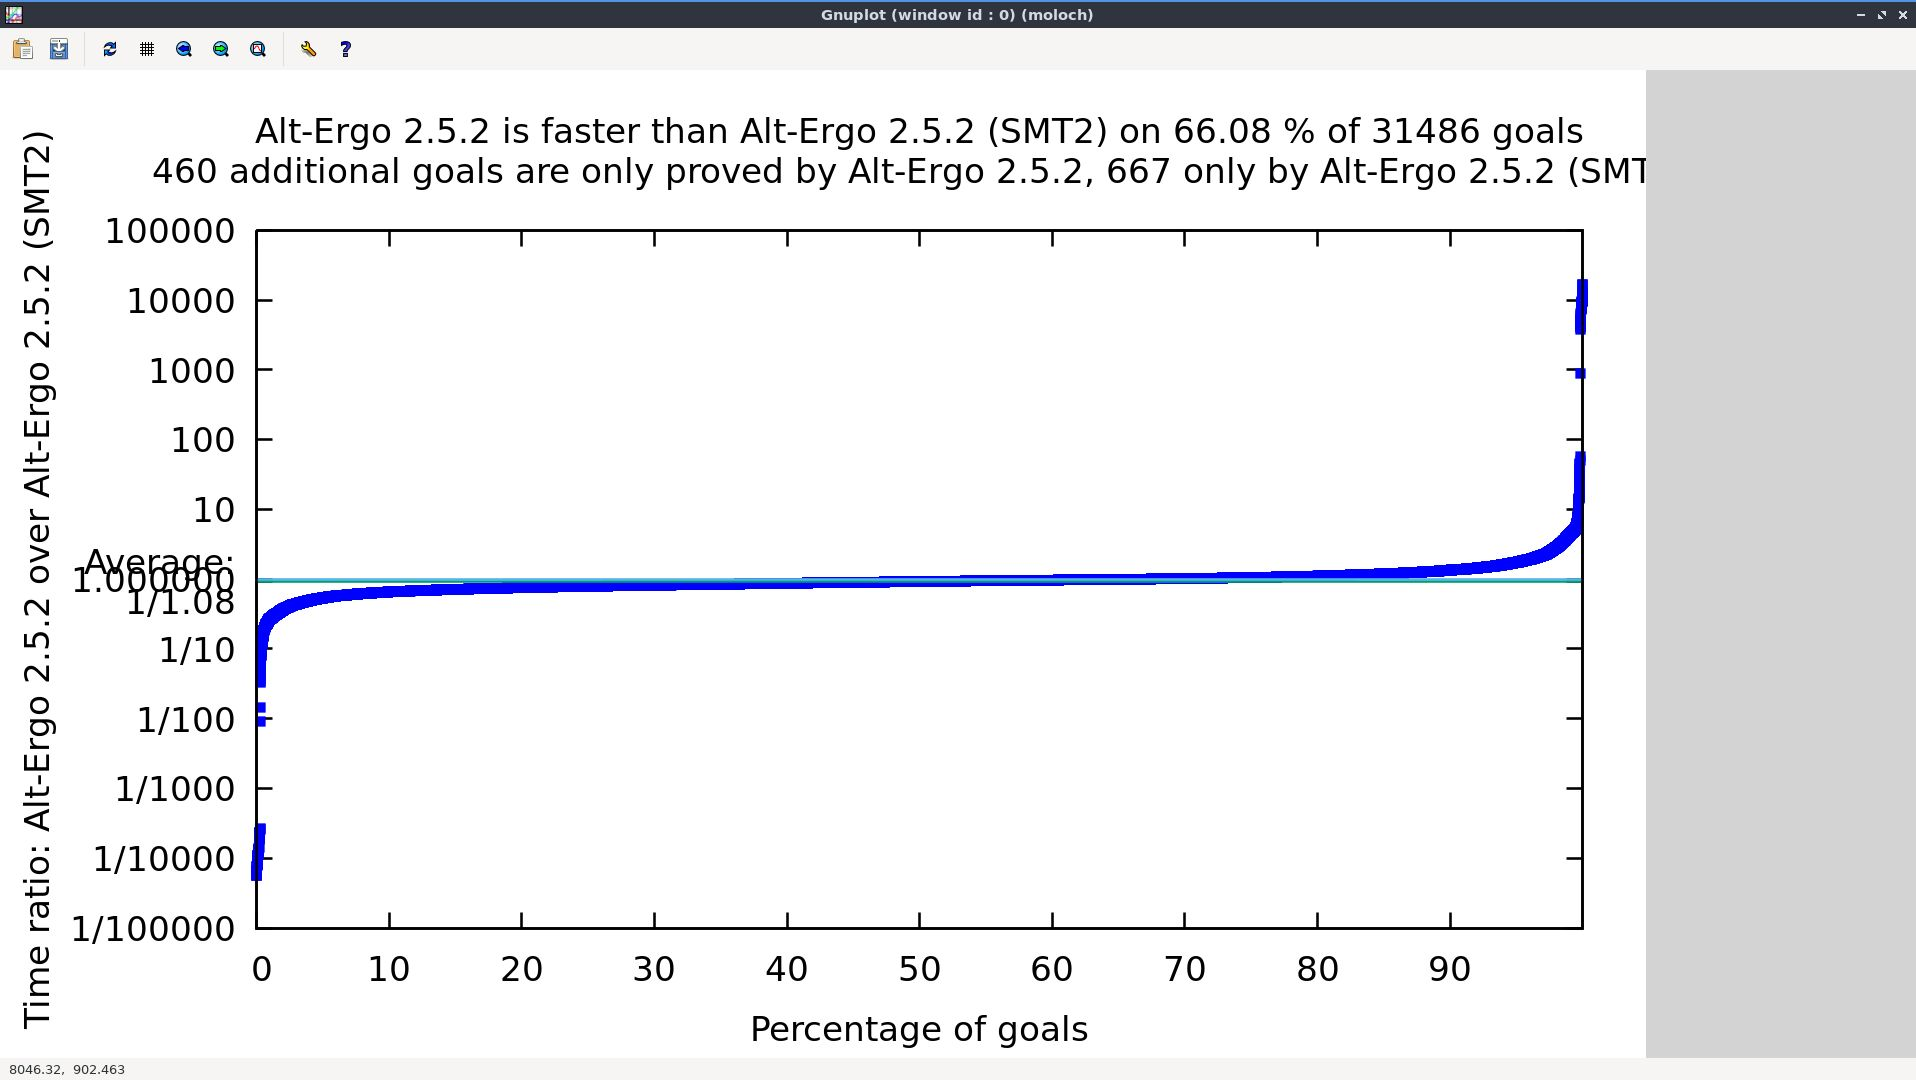
\includegraphics[width=\textwidth]{alt_ergo_smt.jpg}
  \end{center}

\end{frame}

\begin{frame}{Why3 bench/session: future work}

  \begin{itemize}
  \item Meilleures statistiques, par exemple
    \begin{itemize}
    \item Temps médian plutôt que temps moyen
    \item Afficher infos de \why{--graph=hist} aussi avec \why{--provers-stats}
  \end{itemize}

\item Pouvoir comparer des modèles WhyML différents

\item Avoir des statistiques pour les contre-exemples

%\item Constituer plus jeux de tests, tester plus de configurations de prouveurs!

  \begin{block}{Suggestions bienvenues}
    (sous forme de ticket Why3, svp)
  \end{block}

\end{itemize}

\end{frame}

\begin{frame}{Structure des jeux de tests}

  \begin{itemize}
  \item Dans le dépôt github, repertoire livrable (OK?)
    \begin{itemize}
    \item Mais: des fichiers générés sous git c'est pas super...
    \end{itemize}
  \item Besoin d'avoir des fichiers de test + la methode de génération (scripts shell?)
  \item \ldots
  \end{itemize}

  \begin{block}{A faire en réunion}
    Proposer une structure
    \begin{itemize}
    \item Jeu de tests Why3
    \item Jeu de tests Spark
    \item Jeu de tests J3
    \item Jeu de tests Creusot
    \end{itemize}
  \end{block}

  \begin{block}{Objectif ?}
    Avoir des jeux de tests d'ici 6 mois, et des statistiques de référence
  \end{block}

\end{frame}

\end{document}



%%% Local Variables:
%%% mode: latex
%%% TeX-master: t
%%% TeX-PDF-mode: t
%%% mode: flyspell
%%% mode: accents
%%% ispell-local-dictionary: "francais"
%%% End:
